\chapter{Related work}
\label{ch:related_work}
Here we discuss works related to our project.

\section{Automated Game Design}
In this section, we discuss the various works that are related to the automated game design aspect of our project. First, we go over projects that have similar goals to ScriptButler and contrast the differences. In the last section, we delve into the AI perspective of AGD. This perspective is not the focus of our thesis, but it is an important part of AGD.

\subsection{AI-Based Automation}
AI-Based automation is used in two distinct ways in Game Design and we will briefly discuss each. We do not discuss AIs as part of a game but rather AI as a tool for game design and development. Although AI as part of games is an interesting area as they provide additional replayability and randomness to a game. That perspective was briefly covered in our Procedural Content Generation section.

The first way that AI-based automation is used is as a way to support developers in their endeavors through such things as automated mechanics testing. Automated mechanics testing is similar to playtesting in that a player goes through the level insuring that certain actions result in certain level states. However, the method does not provide the ability to analyze the experience. AI-based playtesting is a relatively new area of game design that involves both physical games\cite{10.1145/3102071.3102105} and digital games. The concept is having an algorithm crawl the game's various obstacles and come up with solutions much more methodically than a human could.

The second way that AI-based automation is used is as a way to support the designers in their endeavors through such things as AI-generated content. This can include things like automatically generating levels based on game mechanics, generating game mechanics based on a preset, or generating a narrative based on rules. In these cases, the AI system influences the mechanics and aesthetics of the game. Game design provides context to the AI which in turn generates affordances for the game based on the domain of the game as can be seen in Figure \ref{fig:ai-based game design}.

\begin{figure}[!t]
    \centering
    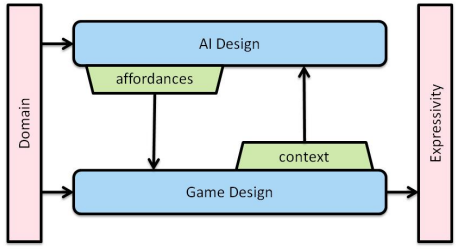
\includegraphics[width=0.66\textwidth]{images/AI-based game desig.png}
    \caption{Illustrating the process of AI-based game design (adapted from Eladhari\cite{Eladhari2011AIBasedGD})}
    \label{fig:ai-based game design}
\end{figure}

This concept is well illustrated in the paper by Eladhari\cite{Eladhari2011AIBasedGD} which discusses the concepts of context and affordances before relating them to the iterative design loop. Another paper by Eladhari\cite{10.1145/1501750.1501798} discusses a technical framework called \textit{Mind Module} which aims to model emotion in the world of games. This module generates parts of the game based on the player responses.

\subsection{Examples of AGD}
\paragraph{PlaySpecs} A paper by Osborn et al.\cite{osborn2015playspecs} connects the concepts of automated analysis with software verification. This is similar to our approach where we apply techniques used in software engineering to perform automated game analysis. The author proposes the tool \emph{Playspecs} to test PuzzleScript games. Any puzzle game can define Playspecs conditions that must hold for any found solution on each level. A solution that violates this constraint notifies the developer. However, PlaySpecs requires play traces to analyze. In the paper, this is done by generating solutions using a heuristic search. In other cases, this could be also done manually through playtesting. PlaySpecs' target audience is game engines and engine developers.

\paragraph{Ludoscope} Dormans proposes the tool \emph{Ludoscope} as a way to analyze how level space relates to level missions. They illustrate those concepts in "Adventures in level design"\cite{DBLP:conf/fdg/Dormans10} in the context of a \emph{The Legend of Zelda} game. Ludoscope is a general-purpose tool for generating content using transformational grammars. Ludoscope is extensible and in a validation follow-up validation experiment by Dormans\cite{Dormans2013CombinatorialAE}. The tool can then be extended based on project-specific needs. Ludoscope touches on the concepts of automated game design and procedural content generation. Game designers define constraints for generation and the tool provides feedback after the generation. ScriptButler does not generate any content but it is similarly extensible. 

\paragraph{Micro-Machinations} \emph{Micro-Machinations}\cite{DBLP:conf/sle/KlintR13} (MM) is a textual and visual programming language that extends \emph{Machinations}. Van Rozen and Dorman\cite{DBLP:conf/fdg/RozenD14} propose a live programming approach as an embeddable MM library. This approach of rapid prototyping is similar to our approach with ScripButler. However, our approach does not focus on providing alternative methods for creating those games, only feedback on existing code.



\section{PuzzleScript}
PuzzleScript's popularity and features generate a lot of interest for developers looking to research game design. Because of that, a few other works have been done relating to it. In this section, we present these different works and how they relate to our project.

We want to mention the project by GitHub user vexorian\cite{puzzlescript-bfs} which implements Breath-First search as a PuzzleScript game. It does not necessarily relate to this project but shows an interesting way of applying Puzzlescript in education. Users can create their own levels to test how breath-first search interacts with it and study the Rules of the game to understand how it works in theory. 

The project repository recommends running the project on a fork of PuzzleScript which includes additional features\footnote{\url{https://pancelor.com/PuzzleScript/editor.html}} such as the ability to jump to specific levels. It is another of those forks that extend PuzzleScript with very small specific changes to suit their needs\cite{pancelor}.

\subsection{Other Implementations}
Here we compare the features of different implementations of PuzzleScript which we previously discussed in Section \ref{ch:background}. The comparison can be seen in Table \ref{fig:feature_comparison_rw}. The bottom line is that none of these implementations really focus on changing the design process of PuzzleScript game, they are all focused on simply reimplementing PuzzleScript in a different language for convenience. The Rust implementation specifically mentions that it handles rules differently from the original engine but that seems to cause issues. We did not compare PatternScript\cite{PatternScript} because it is an implementation of PuzzleScript in JavaScript, something we already knew possible since the original implementation is in JavaScript.

\begin{figure}[!t]
    \centering
    \caption{Feature Comparison between the original implementation and other implementations.}
\begin{tabular}{p{2cm}|p{3cm}|p{2cm}|p{2cm}|p{2cm}|p{2cm}}
\small
    \textbf{Category} & \textbf{Feature}    & \textbf{JavaScript}   & \textbf{C++}                 & \textbf{Rust}           & \textbf{C}                    \\ \hline
    \textit{Editor}   & Text Editor         & Yes                   & No                           & No                      & No                            \\
                      & Syntax Coloring     & Yes                   & No                           & No                      & No                            \\
                      & Messages            & No                    & No                           & No                      & No                            \\
                      & Game frame          & Yes                   & No                           & No                      & No                            \\
                      & Autocomplete        & Yes                   & No                           & No                      & No                            \\
                      & Export              & Yes                   & No                           & No                      & No                            \\
                      & Share               & Yes                   & No                           & No                      & No                            \\
                      & Save states         & Yes                   & No                           & No                      & No                            \\
                      & Keyboard control    & Yes                   & No                           & Yes                     & Yes                           \\
                      & Debug               & Yes                   & No                           & No                      & No                            \\
    \textit{Parser}   & Error Checking      & Yes                   & Yes                          & Yes                     & Yes                           \\
                      & Grammar             & Implicit              & Implicit                     & No, JSON-based          & Implicit                      \\
    \textit{Checker}  & Error Checking      & N/A                   & N/A                          & No                      & Yes but no line number        \\
                      & Errors              & 101                   & 101                          & N/A                     & 101                           \\
                      & Warnings            & 19                    & 19                           & N/A                     & 19                            \\
                      & Error Isolation     & No, cascades          & No, cascades                 & N/A                     & No                            \\
    \textit{Compiler} & Error Checking      & Yes                   & Yes                          & N/A                     & Yes                           \\
                      & Prelude             & Yes                   & Mostly missing               & Yes                     & Yes                           \\
                      & Objects             & Yes                   & Implemented                  & Yes                     & Yes                           \\
                      & Legend              & Yes                   & Implemented                  & Yes                     & Yes                           \\
                      & Sounds              & Yes                   & No                           & Yes                     & No                            \\
                      & Layers              & Yes                   & Yes                          & Yes                     & Yes                           \\
                      & Rules               & Yes                   & Yes, commands missing   & Yes                     & Yes, mostly working           \\
                      & Win Conditions      & Yes                   & Yes                          & Yes                     & Yes                           \\
                      & Levels              & Yes                   & Yes                          & Yes                     & Yes                           \\
    \textit{Engine}   & Randomness          & Yes                   & No                           & Yes                     & Yes                           \\
                      & Rigid Bodies        & Yes                   & No                           & Yes                     & No                            \\
                      & Real time           & Yes                   & No                           & Yes                     & Yes                           \\
                      & Rule Loops          & Yes                   & No                           & Yes                     & No                            \\
    \end{tabular}
    \label{fig:feature_comparison_rw}
\end{figure}

\subsection{Solvers}
Here we discuss how solving algorithms are used in PuzzleScript. We have found three instances of AI being applied to PuzzleScript with the purpose of automated playthrough.

A paper by Chong-U Lim and D. Fox Harrell\cite{6932896}\footnote{\url{https://github.com/icelabMIT/PuzzleScriptAI}} present a repository with a series of algorithms for solving PuzzleScript levels. However, the most interesting part is that the project is not simply implementing an AI but provides an interface for anyone to implement their own algorithms. The similarity between this paper and our own project is interesting, except that instead of providing a wrapper for PuzzleScript we provide our own implementation with its own endpoints. A project by Lauren Cunningham\cite{PuzzleScriptSolver} uses the extension to implement a Monte Carlo Tree Search and shows how exactly one can use such tools. 

A project hosted by GitHub user marcosdon\cite{PuzzleScriptWithSolver} is a full PuzzleScript editor and as such is very easy to play around with. The project adds a "Solve" button to the top bar which runs through the level extremely fast and provides a series of movements to solve the level. It only provides one solution, however, so when there are multiple ways to solve a level, it should be interesting to see which one it picks. The interface uses PuzzleScript's code but the algorithm itself is quite simple, as such it gets easily stuck. We tested on the game we selected for our case study and it became essentially stuck at the third level, always getting caught by the guards. Perhaps it needs more PuzzleScript-specific awareness. This is where the previous project is useful as it allows users to extend the algorithms themselves.



